\documentclass[11pt]{article}
\usepackage{amsmath, amssymb, amsthm}
\usepackage{geometry}
\usepackage{setspace}
\usepackage{minted}
\usepackage{graphicx}
\usepackage{url}

\geometry{margin=1in}
\setlength{\parindent}{0pt}

\title{Homework 1}
\author{Andrew Wang}
\date{27 January 2026}

\begin{document}
\maketitle

\section*{Problem 1}

Let $f : \mathcal{C} \to \mathbb{R}$ be a differentiable and convex function defined on a convex set $\mathcal{C} \subset \mathbb{R}^d$. Consider the constrained optimization problem
\begin{equation}
\min_{x \in \mathcal{C}} f(x).
\end{equation}

\subsection*{(a)}

Show that a point $x^*$ is a solution to (1) if and only if there exists a subgradient
$v \in \partial f(x^*)$ such that
\[
v^\top (y - x^*) \ge 0 \quad \text{for all } y \in \mathcal{C}.
\]

\hrulefill

\textbf{Proof ($\Rightarrow$)}

Assuming that $x^\star$ is a minimizer,
\begin{equation}\label{1a1}
    f(y) - f(x^\star) \ge 0 \quad \forall y \in C.
\end{equation}

Now consider $\phi(\alpha) = f(x^* + \alpha(y-x)) \quad \alpha \in [0,1]$. Because $C$ is convex, $x^* + \alpha(y-x) \in C \quad \forall y$. Therefore using \ref{1a1} we know
\begin{align*}
    \phi(\alpha) - \phi(0) &\geq 0 \\
    \Rightarrow \phi'(0^+) \geq 0,
\end{align*}
as $\alpha = 0$ is a one-sided minimizer of $\phi$ over $[0,1]$

We can find
\[
\phi'(0^+) = \nabla f(x^* + \alpha(y-x))^\top |_{\alpha=0} (y-x^*),
\]

so
\begin{align*}
    \quad \nabla f(x^*)^\top (y-x^*) \geq 0.
\end{align*}

And since $f$ is differentiable and convex,
\[
f(y) \geq f(x^*) + \nabla f(x^*)^\top (y - x^*),
\]
which from the definition of the subdifferential implies that $\nabla f(x^*) \in \partial f(x^*)$. Therefore we can always choose some $v = \nabla f(x^*)$ to satisfy the condition $v^\top (y - x^\star) \ge 0 \quad \forall y \in C.$

\textbf{Proof ($\Leftarrow$)} 

Assume that there exists $v \in \partial f(x^\star)$ such that $v^\top (y - x^\star) \ge 0$ for all $y \in C$. Because $v \in \partial f(x^*)$,
\begin{equation}\label{1a2}
    f(y) \ge f(x^\star) + v^\top (y - x^\star), 
\end{equation}
, and therefore
\[
f(y) \ge f(x^\star) \quad \forall y \in C,
\]
so $x^\star$ is a minimizer.

\hrulefill

\subsection*{(b)}
If $\mathcal{C} = \mathbb{R}^d$, show that $0 \in \partial f(x^*)$, where $x^*$ is a solution
to (1).

\hrulefill

\textbf{Proof}

If $\mathcal{C} = \mathbb{R}^d$, $x^* - \alpha(y-x^*) \in \mathbb{R}^d \quad \forall \alpha \in [0,1]$. Now let $z = x^* + d$ and $y = x^* - d$. Since there is no lower bound on $\mathcal{C}$, it must be that $x^* - \alpha(z - x^*) \in \mathbb{R}^d$ as well. From part a we know that
\begin{align*}
    \begin{cases}
        v^\top (y - x^*) \geq 0 \\
        v^\top (z - x^*) \geq 0
    \end{cases} \\
    \Rightarrow
    \begin{cases}
        v^\top (-d) \geq 0 \\
        v^\top d \geq 0
    \end{cases}\quad,
\end{align*}
which can only be the case if $v = 0$.

\hrulefill

\subsection*{(c)}

Show that $\partial f(x) = \{\nabla f(x)\}$ is a singleton for any $x \in \mathcal{C}$.

\hrulefill

\textbf{Proof}
Since $f$ is convex and differentiable, every $\nabla f(x) \in \partial f(x)$ (from part a). Therefore $\{\nabla f(x)\} \subseteq \partial f(x)$.

For some subgradient $v \in \partial f(x)$, 
\[
f(y) \ge f(x) + v^\top (y - x)
\]
Now consider $y = x + td, \quad t > 0$. Then the above becomes
\[
\frac{f(x + td) - f(x)}{t} \geq v^\top d,
\]
and if we take the limit of the left side as $t \downarrow0$ we get $\lim_{t \downarrow 0} \frac{f(x + td) - f(x)}{t} = \nabla f(x)^\top d$, giving us
\[
\nabla f(x)^\top d \geq v^\top d,
\]
or equivalently $(\nabla f(x) - v)^\top d \geq 0 \quad \forall d$. We can repeat the same argument with $y = x - td$ to show $(\nabla f(x) - v)^\top d \leq 0 \quad \forall d$. Evidently, it must be that $(\nabla f(x) - v) = 0 \quad \Rightarrow \quad \nabla f(x) = v$, that is every subgradient $v = \nabla f(x)$, so the set of subgradients $\partial f(x) \subseteq \{\nabla f(x)\}$. But we already showed $\{\nabla f(x)\} \subseteq \partial f(x)$, so it must be that $\{\nabla f(x)\} = \partial f(x)$.

\hrulefill

\section*{Problem 2}
Let $f : \mathcal{C} \to \mathbb{R}$ be a differentiable function defined on a convex set
$\mathcal{C} \subset \mathbb{R}^d$. Show that if $f$ is $L$-smooth for some $L > 0$, then
\[
f(y) \le f(x) + \nabla f(x)^\top (y - x) + \frac{L}{2}\|y - x\|_2^2
\]
for all $x, y \in \mathcal{C}$.

Show that the converse is also true if additionally $f$ is convex and twice differentiable on
$\mathcal{C}$. That is, the above inequality implies $L$-smoothness for some $L > 0$.

\hrulefill

\textbf{Proof ($\Leftarrow$)}

We want to place a bound on the error term of the first-order Taylor expansion of $f(y)$ around $x$.

We begin by defining $\phi(\alpha) = f(x + \alpha(y-x))$ as in question 1. Then
\begin{align*}
    f(y) - f(x) &= \phi(1) - \phi(0) \\
    &= \int_0^1 \nabla f(x + \alpha (y-x))^\top (y-x) d\alpha \\
    \Rightarrow \quad f(y) &= f(x) + \int_0^1 \nabla f(x + \alpha (y-x))^\top (y-x) d\alpha + \nabla f(x)^\top (y-x) - \nabla f(x)^\top (y-x).
\end{align*}

We also know $\nabla f(x)^\top (y-x) = \int_0^1 \nabla f(x)^\top (y-x)d\alpha$ since the interior of the integral is free of $\alpha$. Therefore, the above becomes
\begin{align}
    f(y) &= f(x) + \int_0^1 \nabla f(x + \alpha (y-x))^\top (y-x) d\alpha + \nabla f(x)^\top (y-x) - \int_0^1 \nabla f(x)^\top (y-x)d\alpha \nonumber \\ 
    &= f(x) + \nabla f(x)^\top (y-x) + \int_0^1 \nabla f(x + \alpha (y-x))^\top (y-x) - \nabla f(x)^\top (y-x)d\alpha \nonumber \\
    &= f(x) + \nabla f(x)^\top (y-x) + \int_0^1 \big[\nabla f(x + \alpha (y-x)) - \nabla f(x)\big]^\top (y-x) d\alpha \label{2.1},
\end{align}

which is pretty much the first-order Taylor expansion but with a different form for the error term. We can apply the Cauchy-Schwarz inequality to the error term to show
\[
\int_0^1 \big[\nabla f(x + \alpha (y-x)) - \nabla f(x)\big]^\top (y-x) d\alpha \leq \|y-x\|_2 \int_0^1 \| \nabla f(x + \alpha (y-x)) - \nabla f(x) \|_2 d\alpha.
\]
We know from L-smoothness that $\| \nabla f(x + \alpha (y-x)) - \nabla f(x) \|_2 \leq L\|\alpha(y-x)\|_2$, so we can simplify the right-hand side above as
\begin{align*}
    \int_0^1 \big[\nabla f(x + \alpha (y-x)) - \nabla f(x)\big]^\top (y-x) d\alpha &\leq \|y-x\|_2 \int_0^1 L\|\alpha(y-x)\|_2 d\alpha \\
    &\leq \|y-x\|_2 L \|y-x\|_2 \int_0^1 \alpha d\alpha \\
    &\leq \frac{L}{2} \|y-x\|_2^2.
\end{align*}
Applying this to \ref{2.1} gives
\[
f(y) \leq f(x) + \nabla f(x)^\top (y-x) + \frac{L}{2} \|y-x\|_2^2
\]

\textbf{Proof ($\Rightarrow$)}

We begin with the second-order Taylor expansion of $f(y)$ about x. Assuming as given that $f$ is convex and twice differentiable in $\mathcal{C}$, then for some $\alpha \in (0,1)$,
\[
f(y) = f(x) + \nabla f(x)^\top (y-x) + \frac{1}{2}(y-x)^\top \nabla^2 f(x+\alpha(y-x)) (y-x).
\]
From here we make use of the fact that, if $f$ is L-smooth and twice-differentiable,  $\nabla^2 f(z) \preceq LI \quad \Rightarrow \quad (y-x)^\top \nabla^2 f(x + \alpha(y-x)) (y-x) \leq L\|y-x\|_2^2$. Thus
\[
f(y) \leq f(x) + \nabla f(x)^\top (y-x) + \frac{L}{2}\|y-x\|_2^2
\].

\hrulefill

\section*{Problem 3}

A differentiable function $f : \mathcal{C} \to \mathbb{R}$ defined on a convex set
$\mathcal{C} \subset \mathbb{R}^d$ is said to be $\lambda$-strongly concave if there exists $\lambda > 0$
such that for all $x, y \in \mathcal{C}$,
\[
f(y) \le f(x) + \nabla f(x)^\top (y - x) - \frac{\lambda}{2}\|x - y\|_2^2.
\]

\subsection*{(a)}

Show that the solution $x^*$ to
\[
\max_{x \in \mathcal{C}} f(x)
\]
is unique if $f$ is $\lambda$-strongly concave.

\hrulefill

\textbf{Proof}

We approach this problem via proof by contradiction. Given that $f$ is $\lambda$-strongly concave, then for all $x \in \mathcal{C}$,
\[
f(x^*) \leq f(x) + \nabla f(x)^\top (x^* - x) - \frac{\lambda}{2}\|x^* - x\|_2^2.
\]

Now assume that $x^*$ is not the unique solution, that is $\exists x \neq x^* \in \mathcal{C}$ such that $f(x) = f(x^*)$.

Then, from strong concavity, we also have
\[
f(x) \leq f(x^*) + \nabla f(x^*)^\top (x - x^*) - \frac{\lambda}{2}\|x - x^*\|_2^2.
\]

From these two inequalities,
\begin{align*}
    \nabla f(x)^\top (x^* - x) - \frac{\lambda}{2}\|x^* - x\|_2^2 &\geq  - \nabla f(x^*)^\top (x - x^*) + \frac{\lambda}{2}\|x - x^*\|_2^2 \\
    \Rightarrow \quad \nabla f(x)^\top (x^* - x) + \nabla f(x^*)^\top (x - x^*) &\geq \lambda\|x^* - x\|_2^2
\end{align*}

From problem 1 part a, we know that if $x = \arg \max_{x \in \mathcal{C}} f(x)$, then $\exists v \in \partial f(x^*)$ such that $v^\top (y - x) \leq 0 \quad \forall x \in \mathcal{C}$; from problem 1 part c we know that $\partial f(x) = \{\nabla f(x)\}$. Thus problem 1 informs us that $\nabla f(x)^\top (y - x) \leq 0$. We can apply this first-order condition to the above to show that, since $x$ and $x^*$ are both solutions,
\[
\begin{cases}
    \nabla f(x)^\top (x^* - x) \leq 0 \\
    \nabla f(x^*)^\top (x - x^*) \leq 0
\end{cases} \quad.
\]

Therefore $\lambda\|x^* - x\|_2^2 \leq 0$, and since $\lambda > 0$, it must be that $\|x^* - x\|_2^2 \leq 0$, which in turn means $x^* - x = 0 \quad \Rightarrow \quad x^* = x$. This contradicts our assumption that $x^*$ is not unique. This proves uniqueness of the solution.

\hrulefill

\subsection*{(b)}

For an $\varepsilon$-approximate solution $x_\varepsilon$ with
$f(x_\varepsilon) \ge f(x^*) - \varepsilon$, prove that
\[
\|x_\varepsilon - x^*\|_2^2 \le \frac{2\varepsilon}{\lambda}.
\]

\hrulefill

From the strong convexity of $f$,
\[
\frac{\lambda}{2}\|x_\varepsilon - x^* \|_2^2 \leq f(x^*) - f(x_\varepsilon) + \nabla f(x^*)(x_\varepsilon - x^*).
\]
However we know that $f(x^*) \leq f(x_\varepsilon) + \varepsilon$, so 
\[
\frac{\lambda}{2}\|x_\varepsilon - x^* \|_2^2 \leq \varepsilon + \nabla f(x^*)(x_\varepsilon - x^*).
\]

Since $x^* - \arg \max_{x \in \mathcal{C}} f(x) = \arg \min_{x \in \mathcal{C}} g(x)$ where $g(x) = -f(x)$, and $g(x)$ is $\lambda$-strongly convex, we have
\begin{align*}
    g(x_\varepsilon) &\geq g(x^*) + \nabla g(x^*)(x_\varepsilon - x^*) + \frac{\lambda}{2}\|x - x^*\|_2^2\\
    \Rightarrow \quad \nabla g(x^*)^\top(x_\varepsilon - x^*) &\leq g(x_\varepsilon) - g(x^*) - \frac{\lambda}{2}\|x - x^*\|_2^2.
\end{align*}

Once again, we apply the first order condition from problem 1 to show that $\nabla g(x^*)^\top(x_\varepsilon - x^*) \geq 0$, and therefore
\begin{align*}
g(x_\varepsilon) - g(x^*) - \frac{\lambda}{2}\|x - x^*\|_2^2 \geq 0.
\end{align*}

Noting that from the definition of $g$, $g(x_\varepsilon) - g(x^*) = f(x^*) - f(x_\varepsilon) \leq \varepsilon$, we can then show
\begin{align*}
\frac{\lambda}{2}\|x - x^*\|_2^2 &\leq \varepsilon \\
\|x - x^*\|_2^2 &\leq \frac{2\varepsilon}{\lambda}.
\end{align*}

\hrulefill

\subsection*{(b)}

From strong convexity,
\[
\frac{\lambda}{2}\|x-x^\star\|^2 \le f(x) - f(x^\star) \le \varepsilon,
\]
which yields
\[
\|x-x^\star\| \le \sqrt{\frac{2\varepsilon}{\lambda}}.
\]

\hrulefill

\section*{Problem 4}
We consider a binary classification problem with training data
$(x_i, y_i)$, $x_i \in \mathbb{R}^d$, $y_i \in \{\pm 1\}$, $i = 1, \dots, n$.

We use a linear classifier with logistic loss and $\ell_2$ regularization. The objective function is
\[
\hat{w} = \arg\min_{w \in \mathbb{R}^d} f(w),
\]
where
\[
f(w) = \frac{1}{n}\sum_{i=1}^n \log\left(1 + \exp(-y_i x_i^\top w)\right)
+ \frac{\lambda_0}{2}\|w\|_2^2,
\]
and $\lambda_0 > 0$ is the regularization parameter. Let
$X \in \mathbb{R}^{n \times d}$ be the design matrix whose $i$-th row is $x_i^\top$.

\subsection*{(a)}

Derive the explicit form of the gradient $\nabla f(w)$.

\hrulefill

Consider the logistic regression portion:
\begin{align*}
    \nabla \Bigg[ \frac{1}{n}\sum_{i=1}^n \log\left(1+\exp(-y_i x_i^\top w)\right) \Bigg] &= -\frac{1}{n}\sum_{i=1}^n
\frac{y_i x_i}{1+\exp(y_i x_i^\top w)} \\
&= -\frac{1}{n}\sum_{i=1}^n y_ix_i\sigma(-y_ix_i^\top w),
\end{align*}
where $\sigma(t)=\frac{1}{1+e^{-t}}$.

We also have
\[
\frac{\partial}{\partial w}\frac{\lambda_0}{2}\|w\|_2^2 = \lambda_0 w
\]

Then
\[
\nabla f(w) = -\frac{1}{n}\sum_{i=1}^n y_ix_i\sigma(-y_ix_i^\top w) + \lambda_0 w,
\]
where $\nabla f(w)$ is a $d \times 1$ vector.

\hrulefill

\subsection*{(b)}

Derive the Hessian matrix $\nabla^2 f(w)$ and express it in matrix form.

\hrulefill

We first differentiate
\[
\frac{\partial}{\partial w} \Bigg[-\frac{1}{n}\sum_{i=1}^n y_ix_i\sigma(-y_ix_i^\top w)\Bigg] = \frac{1}{n}\sum_{i=1}^n y_i^2x_ix_i^\top\sigma(-y_ix_i^\top w)(1-\sigma(-y_ix_i^\top w)),
\],
where $y_i^2 = 1$ since $y_i \in \{-1,1\}$.

We then differentiate simply
\[
\frac{\partial}{\partial w} \lambda_0 w = \lambda_0 I_{d\times d}
\]

The Hessian is therefore
\[
\nabla^2 f(w)
= \frac{1}{n} X^\top D X + \lambda_0 I_{d\times d},
\]
where $D$ is diagonal with
\[
D_{ii} = \sigma(y_ix_i^\top w)(1-\sigma(y_ix_i^\top w)).
\]

Note that $D_{ii} \le \frac{1}{4}$ as a property of the derivative of the sigmoid function.

\hrulefill

\subsection*{(c)}
Show that $f$ is $L$-smooth and $\alpha$-strongly convex. Write down reasonable values for $L$ and $\alpha$.

\hrulefill

From the previous part (b), we know that $0 \le D_{ii} \le \frac{1}{4}$, so $0 \preceq D \preceq \frac{1}{4}I$. We continue this via
\[
\lambda_0 I \preceq \nabla^2 f(w) \preceq \frac{1}{4n} X^\top X + \lambda_0I,
\]
so $f$ is $\alpha$-strongly convex with $\alpha = \lambda_0$ and $f$ is L-smooth with a reasonable value for L being
\[
L = \frac{1}{4n}\lambda_{\max}(X^\top X) + \lambda_0,
\]
where $\lambda_{max}$ is the maximum eigenvalue for the empirical covariance matrix $\frac{1}{n}X^\top X$, which I believe can be computed algorithmically.

\hrulefill

\subsection*{(d)}

What is the number of iterations required to achieve $\varepsilon$-suboptimality? Express the answer using $O(\cdot)$ notation and your choices of $L$ and $\alpha$.

\hrulefill

Choosing step size $\eta = 1/L$ guarantees convergence of gradient descent to an $\varepsilon$-suboptimal solution at rate $O\big(\frac{1}{\eta \alpha} \log(\frac{1}{\varepsilon})\big) = O\bigg(\big(\frac{1}{4\lambda_0}\lambda_{max}(\frac{1}{n}X^\top X) + 1\big)\log(\frac{1}{\varepsilon})\bigg)$.

\subsection*{(e)}
Let $d = 50$, $n = 100$, and $\lambda_0 = 1$. Generate data as follows:
\begin{enumerate}
\item $w_{\text{opt}} = (1, \dots, 1)^\top \in \mathbb{R}^d$;
\item $X \in \mathbb{R}^{n \times d}$ has i.i.d.\ standard normal entries;
\item $z = X w_{\text{opt}} \in \mathbb{R}^n$ and
\[
p_i = \frac{1}{1 + e^{-z_i}};
\]
\item $Y \in \{\pm 1\}^n$ with independent entries and
$\mathbb{P}(y_i = 1) = p_i$.
\end{enumerate}

Initialize gradient descent with $w_0 = (10, \dots, 10)^\top$.
Take $L = 100$. Implement gradient descent and plot the function values for the first 100 iterations using a semi-log plot.

\hrulefill

I present the required plot in \ref{fig:4e}. The code for this is in the Appendix.

\begin{figure}[ht]
    \centering
    \caption{}
    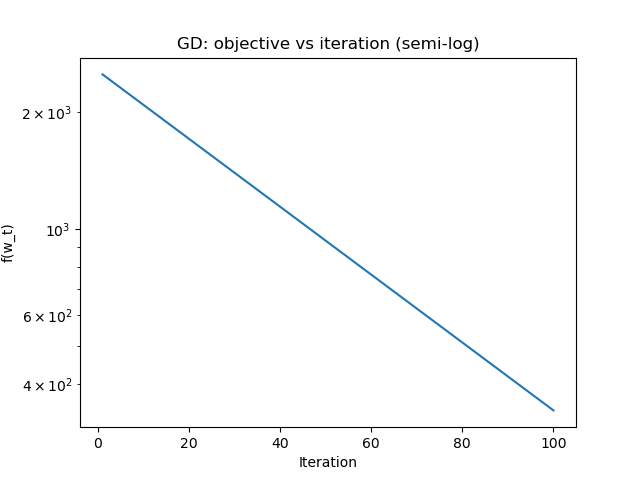
\includegraphics[width=0.7\linewidth]{HW1Q4e.png}
    \label{fig:4e}
\end{figure}

\hrulefill

\subsection*{(f)}
Implement Nesterov’s accelerated gradient descent:
\[
w_{t+1} = w_t - \eta \nabla f(x_t + \gamma(x_t - x_{t-1})) + \gamma(x_t - x_{t-1}),
\]
where
\[
\gamma = \frac{\sqrt{L/\alpha} - 1}{\sqrt{L/\alpha} + 1}.
\]
Plot the function values for the first 100 iterations on the same plot.
Use $L = 100$ and $\alpha = 1$.

\hrulefill

I present the required plot in \ref{fig:4f}. The code for this is in the Appendix.

\begin{figure}[ht]
    \centering
    \caption{}
    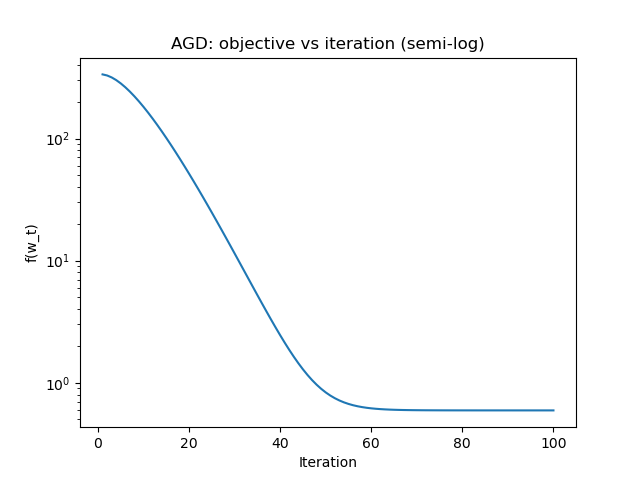
\includegraphics[width=0.7\linewidth]{HW1Q4f.png}
    \label{fig:4f}
\end{figure}

\hrulefill

\section*{Problem 5}

The problem descriptions and code notebook can be downloaded from:
\url{https://colab.research.google.com/drive/1c-maBRpm8IyQyM9fw3B4nORiTDornu8_?usp=sharing}

Finish the programming parts inside the notebook and answer the following:

\subsection*{(a)}
What is the final validation accuracy in Part 6?

\hrulefill

\textbf{My code can be found attached}. My final validation accuracy in Part 6 is 0.94, and the decision boundary is included in \ref{fig:5p7}

\begin{figure}[ht]
    \centering
    \caption{}
    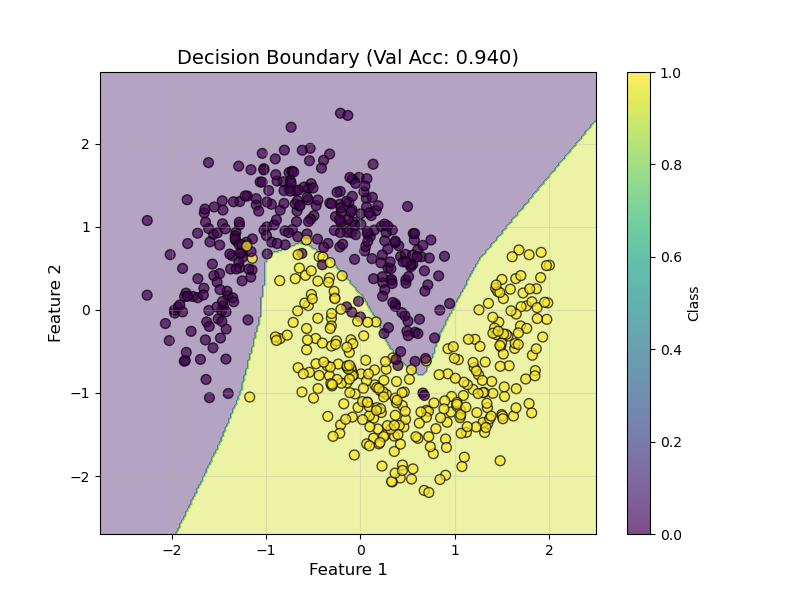
\includegraphics[width=0.7\linewidth]{HW1Q5p7}
    \label{fig:5p7}
\end{figure}

\hrulefill

\subsection*{(b)}
Include all the generated plots from Parts 6--9.

\hrulefill

I include the other plots generated here.

\begin{figure}[ht]
    \centering
    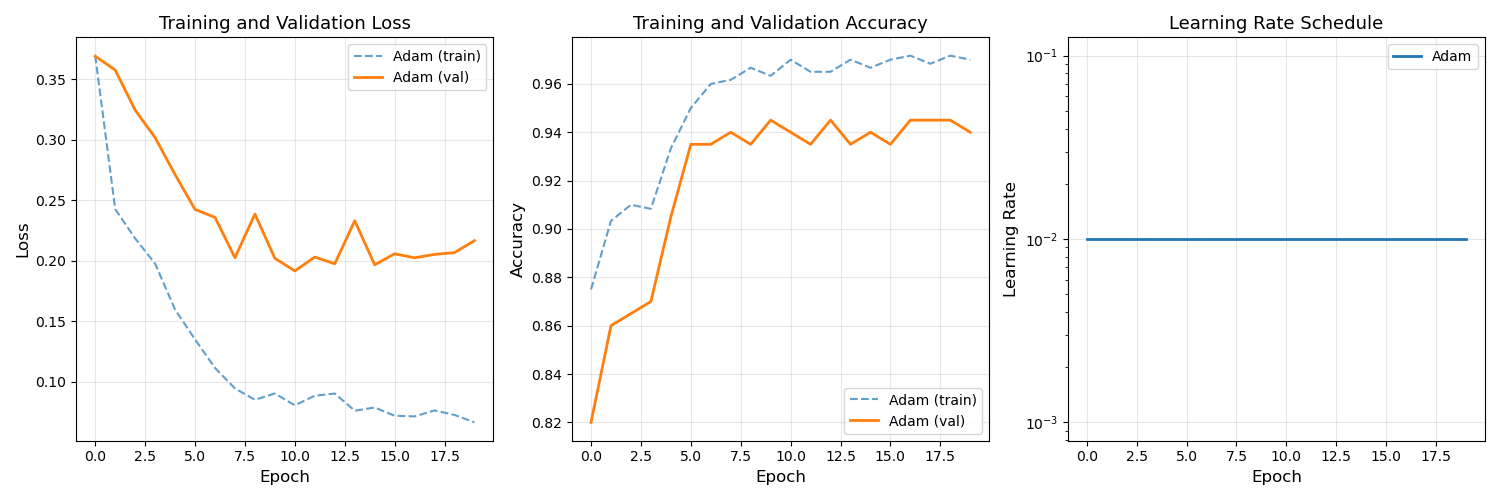
\includegraphics[width=1\linewidth]{HW1Q5.png}
\end{figure}

\begin{figure}[ht]
    \centering
    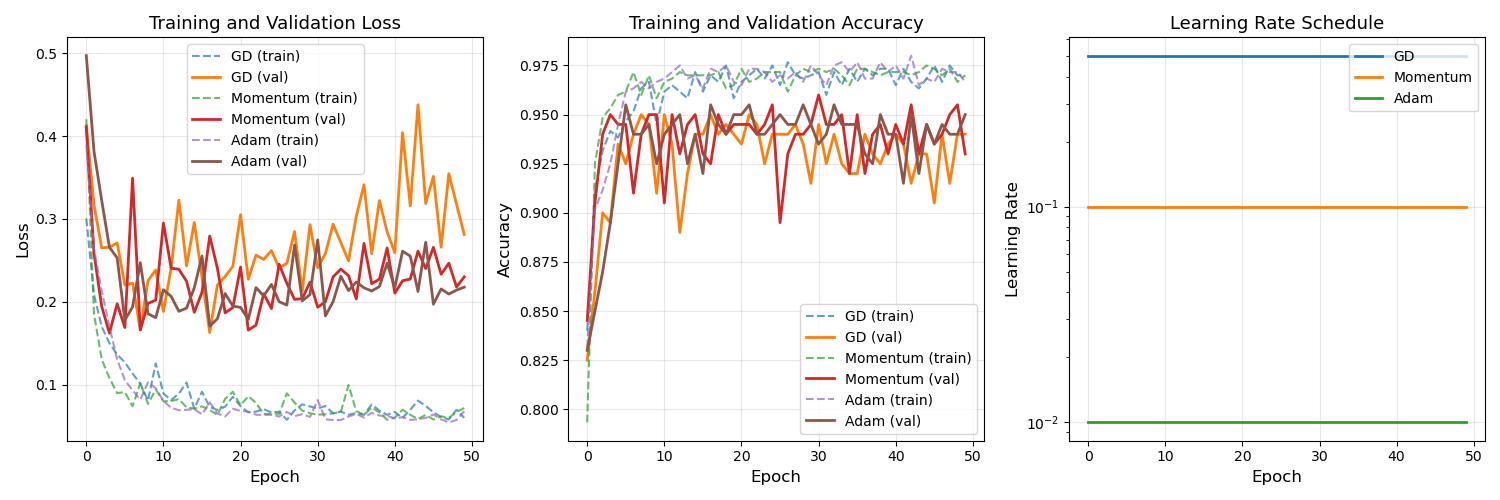
\includegraphics[width=1\linewidth]{HW1Q5p8.png}
\end{figure}

\newpage

\section*{Appendix}

\subsection*{Problem 4(e), 4(f)}

Implement Gradient Descent and Nesterov's Accelerated Gradient Descent.

\inputminted{python}{STAT538_HW1_Q4.py}

\end{document}
